
\section{Funkfernschreiben}
\label{section:funkfernschreiben}
\begin{frame}%STARTCONTENT

\frametitle{Funkfernschreiber}
\begin{columns}
    \begin{column}{0.48\textwidth}
    
\begin{figure}
    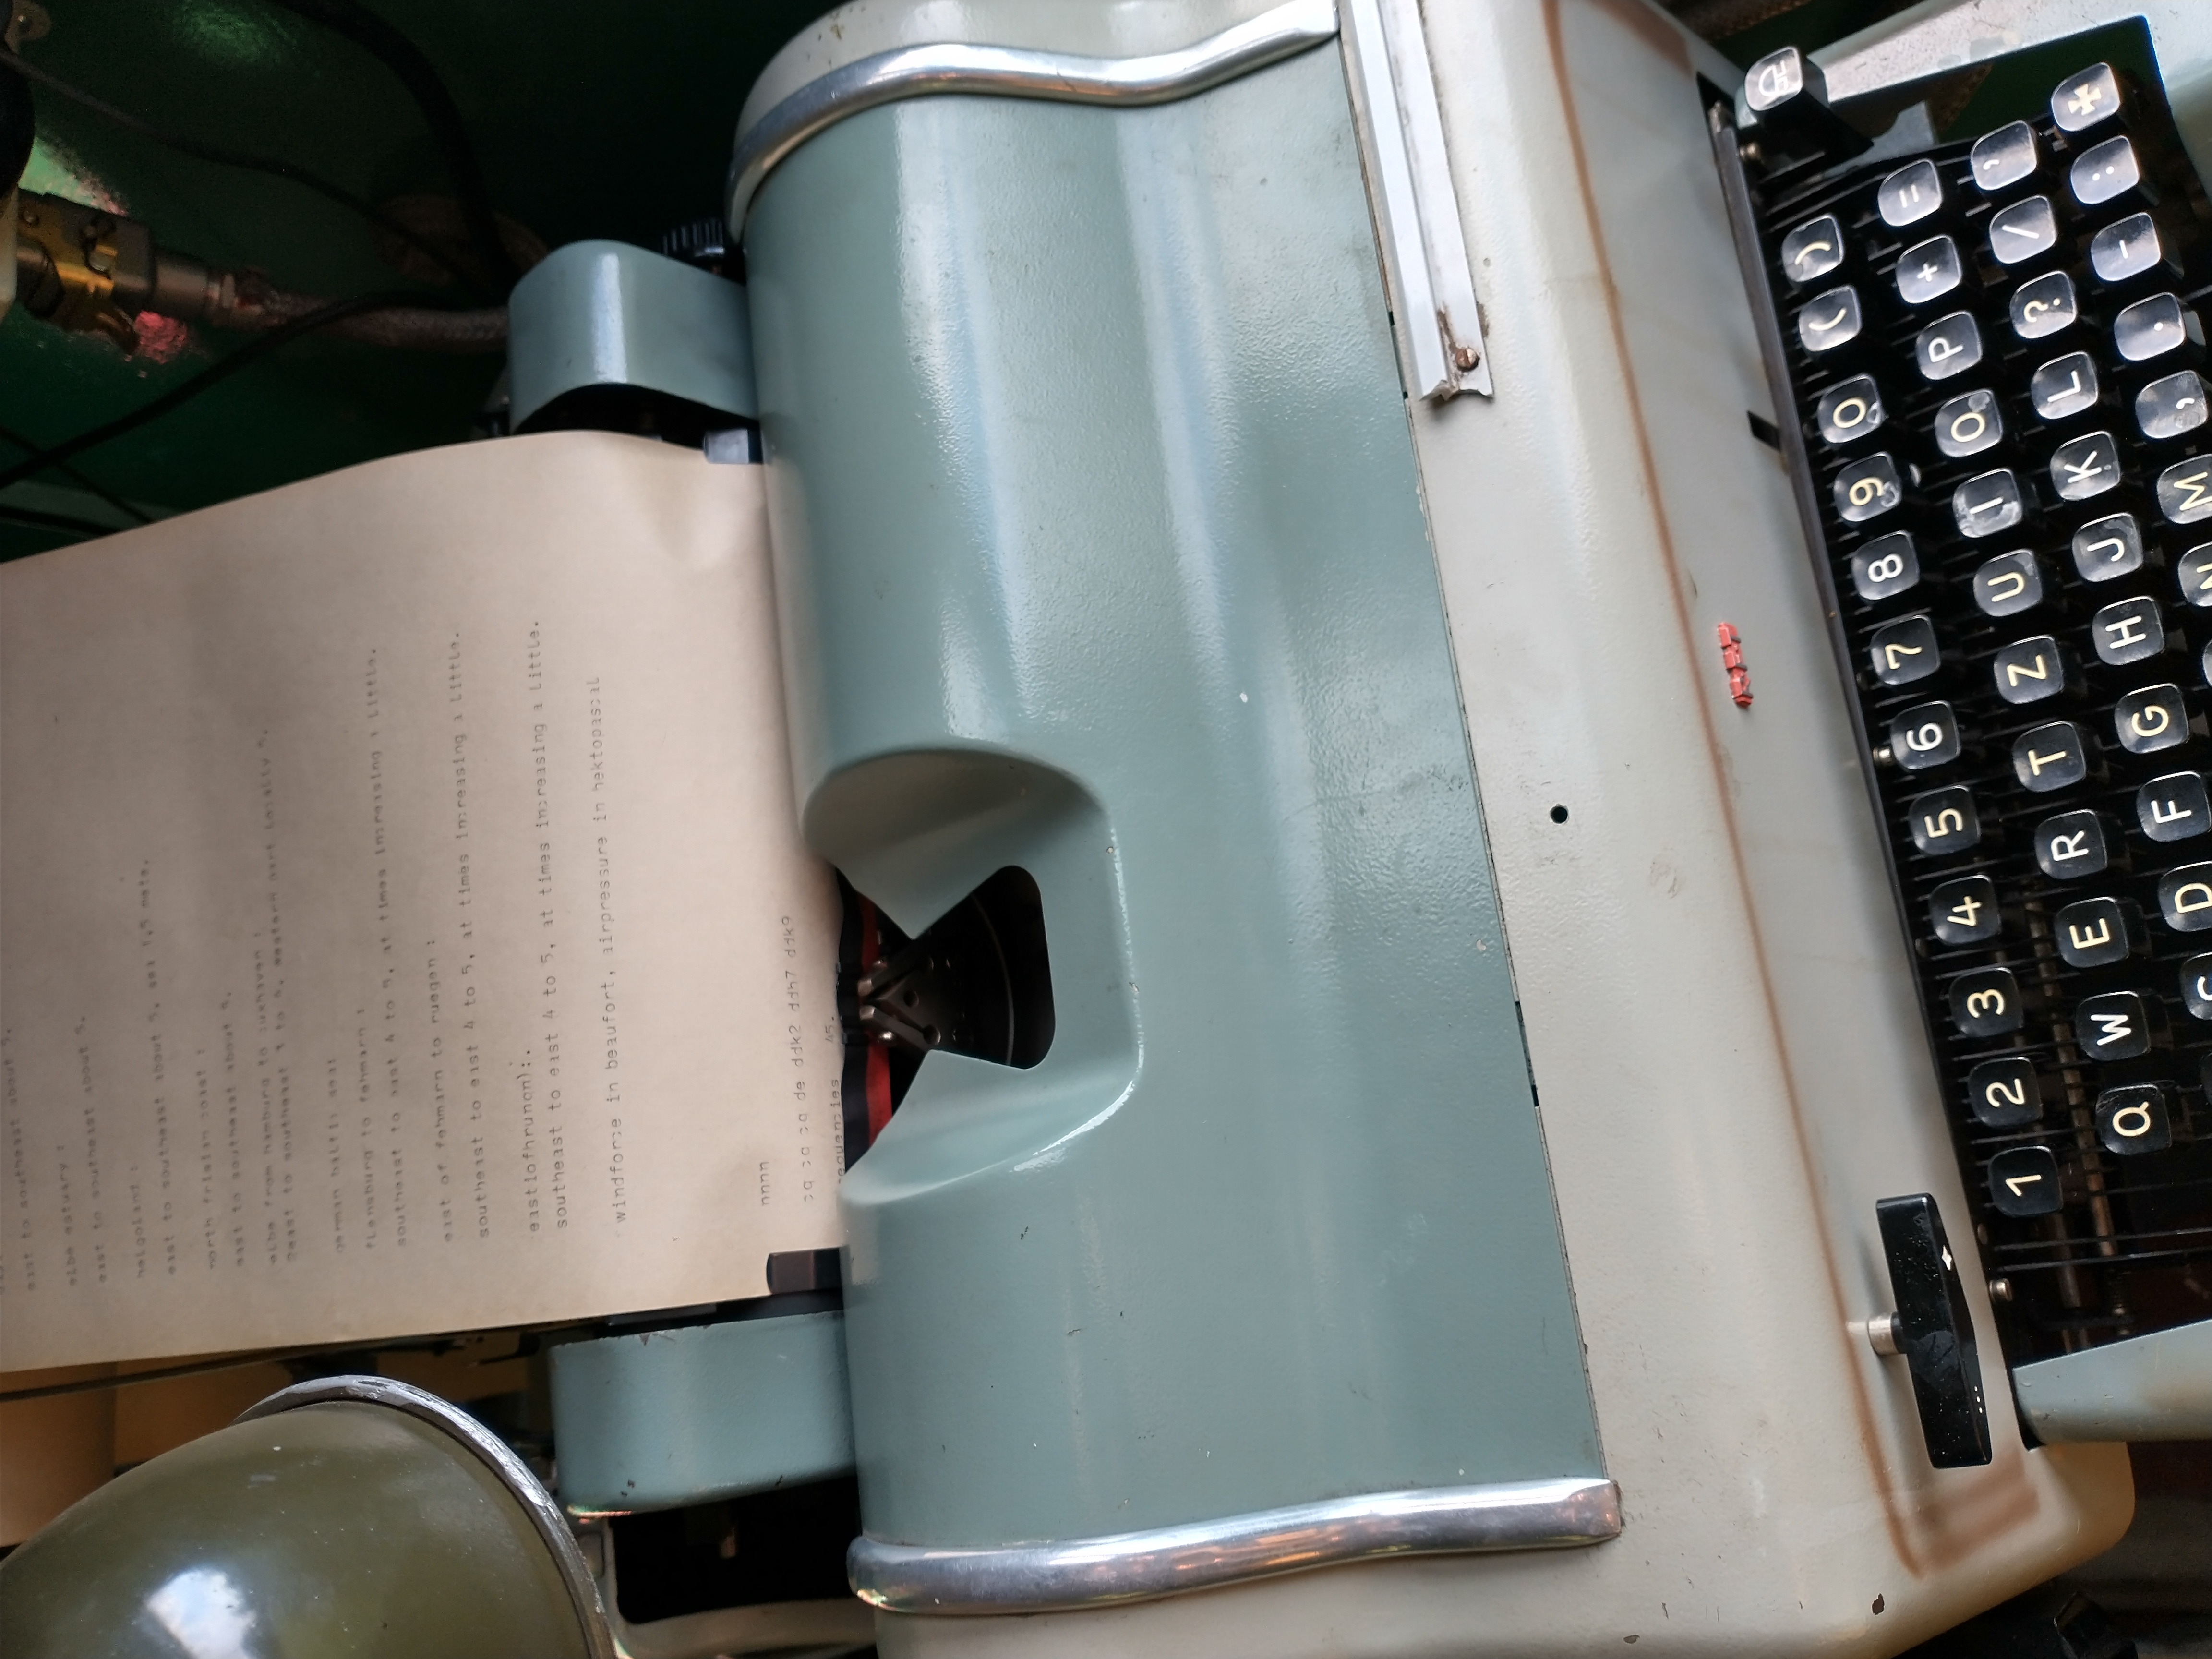
\includegraphics[width=0.85\textwidth]{foto/92}
    \caption{\scriptsize Funkfernschreiber}
    \label{n_computersteuerung_funkfernschreiber}
\end{figure}

    \end{column}
   \begin{column}{0.48\textwidth}
       Die Abkürzung RTTY stammt von \emph{radio teletype}


   \end{column}
\end{columns}

\end{frame}

\begin{frame}
\frametitle{Betrieb}
\begin{columns}
    \begin{column}{0.48\textwidth}
    \begin{itemize}
  \item Beide Funkpartner nutzen das gleiche Übertragungsverfahren (z.B. JS8, PSK, RTTY)
  \item Gleiche Parameter müssen gesetzt sein
  \end{itemize}

    \end{column}
   \begin{column}{0.48\textwidth}
       \begin{itemize}
  \item Verwendung von betrieblichen Abkürzungen und Q-Gruppen
  \item Mehr Informationsgehalt pro Zeiteinheit
  \end{itemize}

   \end{column}
\end{columns}

\end{frame}

\begin{frame}In einem Gespräch sieht dieses folgendermaßen aus:
    \pause\QSOown{CQ CQ CQ DE DL2AB DL2AB DL2AB PSE K}\pause\QSOother{DL2AB DE DL1PZ K}\pause\QSOown{DL1PZ DE DL2AB = UR RST 599 599 = DL1PZ DE DL2AB K}\pause\QSOother{DL2AB DE DL1PZ = TNX RPRT, UR 479 479 BK}\pause\QSOown{BK QSL = VY 73 DE DL2AB SK}\pause\QSOother{R 73 DE DL1PZ SK}

\end{frame}

\begin{frame}
\begin{columns}
    \begin{column}{0.48\textwidth}
    \begin{table}
\begin{DARCtabular}{ll}
     Abkz.  & Bedeutung   \\
     BK  & Unterbrechung der Sendung; Formlose Übergabe   \\
     CQ  & Allgemeiner Anruf (vom Englischen \enquote{Seek You})   \\
     DE  & von   \\
     K  & Aufforderung zum Senden   \\
     PSE  & Bitte (vom Englischen \enquote{Please})   \\
     QSL  & Ich bestätige den Empfang   \\
     R  & Received (Empfangsbestätigung)   \\
     RPRT  & Rapport (vom Englischen \enquote{Report})   \\
\end{DARCtabular}
\caption{Betriebliche Abkürzungen in der Telegrafie}
\label{n_funkfernschreiben_abkuerzungen_1}
\end{table}

    \end{column}
   \begin{column}{0.48\textwidth}
       \begin{table}
\begin{DARCtabular}{ll}
     Abkz.  & Bedeutung   \\
     RST  & RST-Rapport   \\
     SK  & Ende der Verbindung (vom Englischen \enquote{Silent Key})   \\
     TNX  & Danke (vom Englischen \enquote{Thanks})   \\
     UR  & du bist (im Sinne von \enquote{dein Signal ist}, vom Englischen \enquote{you are})   \\
     VY  & sehr (vom Englischen \enquote{very})   \\
     73  & viele Grüße   \\
     =  & Trennzeichen   \\
\end{DARCtabular}
\caption{Betriebliche Abkürzungen in der Telegrafie}
\label{n_funkfernschreiben_abkuerzungen_2}
\end{table}

   \end{column}
\end{columns}

\end{frame}

\begin{frame}Teil 1 unseres Beispiel-Gesprächs:
    \pause\QSOown{CQ CQ CQ DE DL2AB DL2AB DL2AB PSE K}\pause\QSOother{DL2AB DE DL1PZ K}
    \pause
    Allgemeiner Anruf von DL2AB -- Bitte Kommen!
    \pause
    DL2AB von DL1PZ -- Kommen!



\end{frame}

\begin{frame}Teil 2 unseres Beispiel-Gesprächs:
    \pause\QSOown{DL1PZ DE DL2AB = UR RST 599 599 = DL1PZ DE DL2AB K}\pause\QSOother{DL2AB DE DL1PZ = TNX RPRT, UR 479 479 BK}
    \pause
    DL1PZ von DL2AB. Dein Signal ist mit dem RST-Wert 599, ich wiederhole, 599. DL1PZ von DL2AB -- Kommen!
    \pause
    DL2AB von DL1PZ. Danke für den RST-Rapport, dein Signal ist 479, ich wiederhole, 479. Zurück zu dir!



\end{frame}

\begin{frame}Teil 3 unseres Beispiel-Gesprächs:
    \pause\QSOown{BK QSL = VY 73 DE DL2AB SK}\pause\QSOother{R 73 DE DL1PZ SK}
    \pause
    Hier bin ich wieder. Ich bestätige den Empfang. Sehr viele Grüße von DL2AB. Ende der Verbindung.
    \pause
    Verstanden. Viele Grüße von DL1PZ. Ende der Verbindung.



\end{frame}

\begin{frame}
\only<1>{
\begin{QQuestion}{NE401}{Was sollten Sie bei der Übertragung eines Textes per Funkfernschreiben beachten?}{Sende- und Empfangsstation müssen das gleiche Übertragungsverfahren (z. B. JS8, PSK, RTTY) und ggf. die gleichen Verfahrensparameter verwenden.}
{Sende- und Empfangsstation müssen die gleiche Zeitzoneneinstellung (z. B. Sommerzeit) aufweisen, damit die Übertragung erfolgreich sein kann.}
{Die Übertragung sollte bevorzugt während der Abend- und Nachtstunden stattfinden, da die Frequenzen tagsüber für Sprechverbindungen freigehalten werden.}
{Die Übertragung sollte bevorzugt mit einem schnellen Verfahren stattfinden, damit die Amateurfunkbänder nicht unnötig belastet werden.}
\end{QQuestion}

}
\only<2>{
\begin{QQuestion}{NE401}{Was sollten Sie bei der Übertragung eines Textes per Funkfernschreiben beachten?}{\textbf{\textcolor{DARCgreen}{Sende- und Empfangsstation müssen das gleiche Übertragungsverfahren (z. B. JS8, PSK, RTTY) und ggf. die gleichen Verfahrensparameter verwenden.}}}
{Sende- und Empfangsstation müssen die gleiche Zeitzoneneinstellung (z. B. Sommerzeit) aufweisen, damit die Übertragung erfolgreich sein kann.}
{Die Übertragung sollte bevorzugt während der Abend- und Nachtstunden stattfinden, da die Frequenzen tagsüber für Sprechverbindungen freigehalten werden.}
{Die Übertragung sollte bevorzugt mit einem schnellen Verfahren stattfinden, damit die Amateurfunkbänder nicht unnötig belastet werden.}
\end{QQuestion}

}
\end{frame}

\begin{frame}
\only<1>{
\begin{QQuestion}{BB101}{Warum werden insbesondere in der Telegrafie (z.~B. CW, JS8, RTTY) betriebliche Abkürzungen und Q-Gruppen verwendet?}{Sie werden als Kennung beim Amateurfunkpeilen genutzt, um die Sender zu kennzeichnen.}
{Der Informationsgehalt einer Aussendung wird verschleiert und ist damit für Unbeteiligte nicht verständlich.}
{Sie werden bei Verbindungen über Amateurfunksatelliten benutzt, um den Dopplereffekt durch kürzere Durchgänge zu vermeiden.}
{Der Betriebsablauf wird vereinfacht und der zu übertragende Informationsgehalt pro Zeiteinheit optimiert.}
\end{QQuestion}

}
\only<2>{
\begin{QQuestion}{BB101}{Warum werden insbesondere in der Telegrafie (z.~B. CW, JS8, RTTY) betriebliche Abkürzungen und Q-Gruppen verwendet?}{Sie werden als Kennung beim Amateurfunkpeilen genutzt, um die Sender zu kennzeichnen.}
{Der Informationsgehalt einer Aussendung wird verschleiert und ist damit für Unbeteiligte nicht verständlich.}
{Sie werden bei Verbindungen über Amateurfunksatelliten benutzt, um den Dopplereffekt durch kürzere Durchgänge zu vermeiden.}
{\textbf{\textcolor{DARCgreen}{Der Betriebsablauf wird vereinfacht und der zu übertragende Informationsgehalt pro Zeiteinheit optimiert.}}}
\end{QQuestion}

}
\end{frame}

\begin{frame}
\only<1>{
\begin{QQuestion}{BB110}{Was bedeutet \glqq R\grqq{} am Anfang eines Durchgangs in Telegrafie?}{Repeat (wiederhole)}
{Received (empfangen)}
{Rapport (Bericht)}
{Readability (Lesbarkeit)}
\end{QQuestion}

}
\only<2>{
\begin{QQuestion}{BB110}{Was bedeutet \glqq R\grqq{} am Anfang eines Durchgangs in Telegrafie?}{Repeat (wiederhole)}
{\textbf{\textcolor{DARCgreen}{Received (empfangen)}}}
{Rapport (Bericht)}
{Readability (Lesbarkeit)}
\end{QQuestion}

}
\end{frame}

\begin{frame}
\only<1>{
\begin{QQuestion}{BB109}{Was bedeutet \glqq K\grqq{} am Ende eines Durchgangs in Telegrafie?}{Unterbrechung der Sendung}
{Aufforderung zum Senden}
{Bitte warten}
{Beendigung des Funkverkehrs}
\end{QQuestion}

}
\only<2>{
\begin{QQuestion}{BB109}{Was bedeutet \glqq K\grqq{} am Ende eines Durchgangs in Telegrafie?}{Unterbrechung der Sendung}
{\textbf{\textcolor{DARCgreen}{Aufforderung zum Senden}}}
{Bitte warten}
{Beendigung des Funkverkehrs}
\end{QQuestion}

}
\end{frame}

\begin{frame}
\only<1>{
\begin{QQuestion}{BB108}{Was bedeutet die Betriebsabkürzung \glqq BK\grqq{} in Telegrafie?}{Beendigung des Funkverkehrs; wird auch zur formlosen Begrüßung genutzt}
{Alles richtig verstanden; wird auch zur schnellen Beendigung eines Funkkontakts genutzt}
{Bitte warten; wird auch zur schnellen Anforderung eines Rapports genutzt}
{Signal zur Unterbrechung einer laufenden Sendung; wird auch zur formlosen Übergabe genutzt}
\end{QQuestion}

}
\only<2>{
\begin{QQuestion}{BB108}{Was bedeutet die Betriebsabkürzung \glqq BK\grqq{} in Telegrafie?}{Beendigung des Funkverkehrs; wird auch zur formlosen Begrüßung genutzt}
{Alles richtig verstanden; wird auch zur schnellen Beendigung eines Funkkontakts genutzt}
{Bitte warten; wird auch zur schnellen Anforderung eines Rapports genutzt}
{\textbf{\textcolor{DARCgreen}{Signal zur Unterbrechung einer laufenden Sendung; wird auch zur formlosen Übergabe genutzt}}}
\end{QQuestion}

}
\end{frame}

\begin{frame}
\only<1>{
\begin{QQuestion}{BE112}{Wie gestalten Sie beispielsweise als \glqq DL2AB\grqq{} einen allgemeinen Anruf in Telegrafie?}{CQ CQ CQ DE DL2AB DL2AB DL2AB pse k}
{CQ CQ CQ FRM DL2AB DL2AB DL2AB pse k}
{QRZ QRZ QRZ DE DL2AB DL2AB DL2AB pse k}
{CQ QRZ CQ QRZ CQ QRZ DE DL2AB DL2AB DL2AB pse k}
\end{QQuestion}

}
\only<2>{
\begin{QQuestion}{BE112}{Wie gestalten Sie beispielsweise als \glqq DL2AB\grqq{} einen allgemeinen Anruf in Telegrafie?}{\textbf{\textcolor{DARCgreen}{CQ CQ CQ DE DL2AB DL2AB DL2AB pse k}}}
{CQ CQ CQ FRM DL2AB DL2AB DL2AB pse k}
{QRZ QRZ QRZ DE DL2AB DL2AB DL2AB pse k}
{CQ QRZ CQ QRZ CQ QRZ DE DL2AB DL2AB DL2AB pse k}
\end{QQuestion}

}
\end{frame}

\begin{frame}
\frametitle{Morsetelegrafie}
\begin{itemize}
  \item Auf die richtige Geschwindigkeit achten
  \item Schnell gegebene Morsezeichen brauchen viel Übung zum Verstehen
  \item Gegenstelle nicht mit der Geschwindigkeit überfordern
  \item Faustregel: \emph{Nicht schneller geben, als man selbst aufnehmen kann}
  \end{itemize}

\end{frame}

\begin{frame}
\only<1>{
\begin{QQuestion}{BE117}{Mit welcher Geschwindigkeit sollten Sie einen Anruf in Morsetelegrafie beantworten? In der Regel antworte ich~...}{mit einem Gebetempo von maximal 60 CPM.}
{mit meiner gewohnten Geschwindigkeit.}
{genauso schnell oder langsamer als der Anruf.}
{mit dem höchsten Tempo, das ich fehlerfrei geben kann.}
\end{QQuestion}

}
\only<2>{
\begin{QQuestion}{BE117}{Mit welcher Geschwindigkeit sollten Sie einen Anruf in Morsetelegrafie beantworten? In der Regel antworte ich~...}{mit einem Gebetempo von maximal 60 CPM.}
{mit meiner gewohnten Geschwindigkeit.}
{\textbf{\textcolor{DARCgreen}{genauso schnell oder langsamer als der Anruf.}}}
{mit dem höchsten Tempo, das ich fehlerfrei geben kann.}
\end{QQuestion}

}
\end{frame}

\begin{frame}
\only<1>{
\begin{QQuestion}{BE118}{Was sollten Sie hinsichtlich der Geschwindigkeit bei Morsetelegrafie beachten? Ich gebe in der Regel~...}{nicht schneller, als ich auch aufnehmen kann, und passe mich an langsamere Stationen an.}
{im international festgelegten Einheitstempo von 12 WPM, um eine automatische Dekodierung zu ermöglichen.}
{so schnell ich kann, damit es nicht zu unnötigen Verzögerungen im Betriebsablauf kommt.}
{in dem Tempo, das mir am besten liegt. Andere müssen sich an mich anpassen.}
\end{QQuestion}

}
\only<2>{
\begin{QQuestion}{BE118}{Was sollten Sie hinsichtlich der Geschwindigkeit bei Morsetelegrafie beachten? Ich gebe in der Regel~...}{\textbf{\textcolor{DARCgreen}{nicht schneller, als ich auch aufnehmen kann, und passe mich an langsamere Stationen an.}}}
{im international festgelegten Einheitstempo von 12 WPM, um eine automatische Dekodierung zu ermöglichen.}
{so schnell ich kann, damit es nicht zu unnötigen Verzögerungen im Betriebsablauf kommt.}
{in dem Tempo, das mir am besten liegt. Andere müssen sich an mich anpassen.}
\end{QQuestion}

}
\end{frame}%ENDCONTENT
